% Created 2013-05-07 Ter 00:37
\documentclass[a4paper]{article}
\usepackage{times}
\usepackage[utf8]{inputenc}
\usepackage[T1]{fontenc}
\usepackage{graphicx}
\usepackage{amssymb}
\usepackage{hyperref}
\linespread{1.5}	% double spaces lines
\usepackage[hmargin=3cm,vmargin=3cm]{geometry}
\usepackage{indentfirst}
\usepackage{amsmath}
\usepackage{amsthm}
\usepackage{sectsty}
\usepackage{enumitem}
\usepackage[brazil]{babel}
\usepackage{placeins} %mantem figuras na secao com \FloatBarrier
\usepackage{fixltx2e} %\textsubscript
\hypersetup{%
    pdfborder = {0 0 0}
}




\begin{document}

\begin{center}


\large{ 
\uppercase{ Universidade Federal do Rio Grande do Sul\\

Instituto de Informática \\

Curso de Ciência da Computação \\

Circuitos Digitais (2014/1)\\
}

Prof. Dr. Marcelo de Oliveira Johann \\

Graduandos: \\ Paulo Renato Lanzarin (228818), Ricardo Gabriel Herdt (160622) \\[1cm]

% Title
\bfseries Relatório do laboratório 05\\[1.0cm]
}

\end{center}
\section{Introdução}

	O experimento consistiu em construir no programa Max Plus II os
circuitos de um meio-somador (\emph{half-adder}, um somador-completo
(\emph{full-adder}) e um somador de 4-bit.  Objetivou-se com isso, além de
obter a necessária familiarização com os recursos do programa, estudar tais
circuitos através da simulação funcional e temporal de suas execuções.


\section{Circuitos}

Foram desenvolvidos três circuitos: meio somador, somador completo e somador de
4 bits.

\subsection{Meio somador (\emph{half-adder})}

$S = \overline{A}B + A\overline{B} = A \oplus B $

$C = A . B$

\begin{table}[h]
\centering
\begin{tabular}{| l | l | l | l |}
	\hline
	A	&B	&S	&C	\\
	\hline
	0	&0	&0	&0	\\
	0	&1	&1	&0	\\
	1	&0	&1	&0	\\
	1	&1	&1	&1	\\
	\hline
\end{tabular}
\caption{Tabela verdade do meio somador}
\end{table}

\begin{figure}[h!]
  \centering
  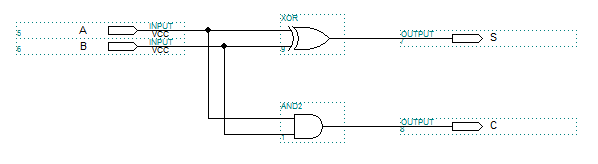
\includegraphics[scale=0.9]{half_adder.png}
  \caption{Diagrama de um meio somador}
\end{figure}



\FloatBarrier
\subsection{Somador Completo (\emph{full-adder})}

$ S = X \oplus Y \oplus C_{in} $

\begin{table}[h]
\centering
\begin{tabular}{| *{3}{p{0.6cm} |} | *{2}{p{0.6cm}|}}
	\hline
	A	&B	&C\textsubscript{in}	&S	&C\textsubscript{out}\\
	\hline
	0	&0	&0	&0	&0	\\
	0	&0	&1	&1	&0	\\
	0	&1	&0	&1	&0	\\
	0	&1	&1	&0	&1	\\
	1	&0	&0	&1	&0	\\
	1	&0	&1	&0	&1	\\
	1	&1	&0	&0	&1	\\
	1	&1	&1	&1	&1	\\
	\hline
\end{tabular}
\caption{Tabela verdade do somador completo}
\end{table}

\begin{figure}[h!]
  \centering
  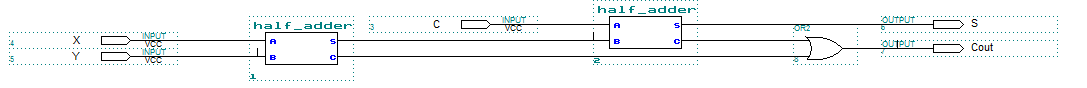
\includegraphics[scale=0.5]{full_adder.png}
  \caption{Diagrama de um somador completo}
\end{figure}


\FloatBarrier
\subsection{Somador de 4 bits}
	Construído com quatro somadores completos, de modo que a saída e o 
vai-um de cada somador servem de entrada para os somadores seguintes.
\begin{figure}[h]
  \centering
  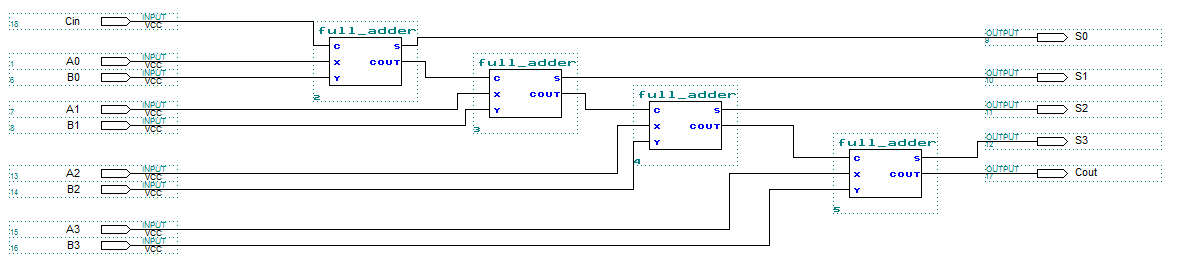
\includegraphics[scale=0.5]{4bit_adder.png}
  \caption{Diagrama de um somador de 4 bits}
\end{figure}

\FloatBarrier
\section{Conclusão}
	Este simples experimento torna nítidas as vantagens de se encapsular 
circuitos inteiros e utilizá-los na construção de estruturas mais complexas,
permitindo ao projetista do circuito raciocinar em níveis mais elevados de
abstração. Este desenvolvimento em etapas fica evidente no uso de uma porta
XOR para o projeto do meio somador, o qual por sua vez é empregado como unidade
lógica na composição do somador completo. Por fim, pôde-se obter facilmente
um somador de 4 bits através da combinação de diversos somadores completos.
	As simulações realizadas, embora careçam de realismo, transmitem uma
noção do comportamento temporal dos circuitos, bem como de suas implicações. [desenvolver]

\end{document}
